\documentclass[../../main.tex]{subfiles}


\begin{document}

\subsection*{(a)}
There are 4982 Applications with an average throughput time of 21.904 as determined using the following Process:\\
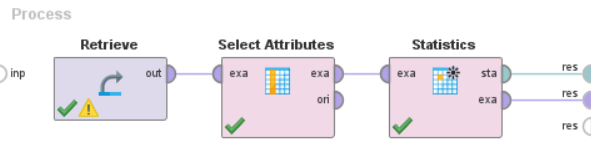
\includegraphics[width=\textwidth]{img/QUESTION_5a_PROCESS_average_throughput_time.png}

Using Celonis Process AI on our Dataset we learn that the most frequent variant (happy path) happens 320 times. This variant can be seen below.\\
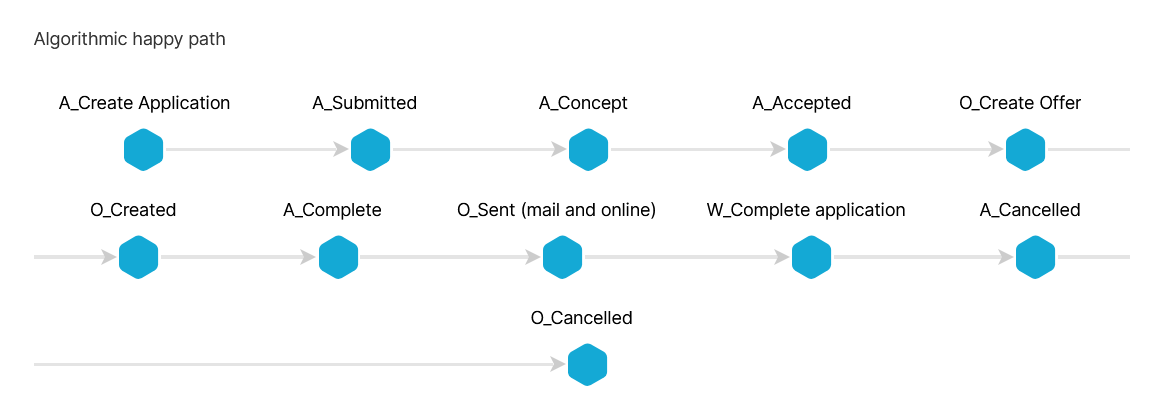
\includegraphics[width=\textwidth]{img/QUESTION_5a_happy_path.png}

The following graph shows the frequency distribution of the throughput times. As one can see they are initially quite high and eventually deteriorate in frequency until the 29-33 Day, where they spike again and after that deteriorate quickly again. The reason for the spike at 29-33 Days is probably that a new month begins/ends at this time. Therefore, many applications will likely be terminated at this time for administrative reasons.\\
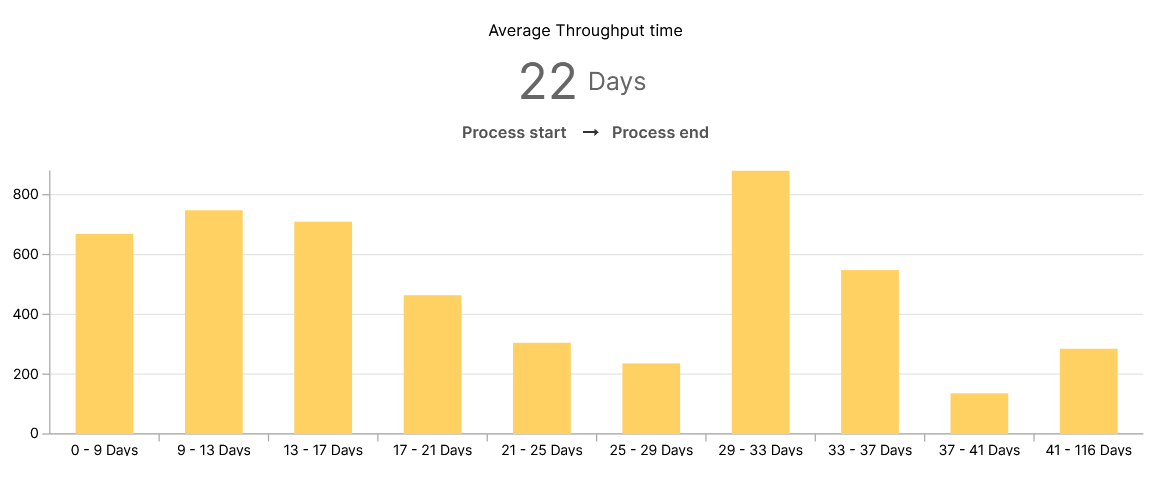
\includegraphics[width=\textwidth]{img/QUESTION_5a_throughput_time_distribution.png}



\subsection*{(b)}
% First item
The BPMN model for cases running under 30 days can be seen below (zoom in to inspect in detail). We created it by starting a new Analysis and opening a new \textit{conformance} sheet. Then we clicked \textit{Mine process model} and in the next window added a new selection for Throughput time under 30. Then we clicked \textit{select all} and \textit{Launch analysis}. We then clicked \textit{View process model} where the model below was displayed and downloadable.\\
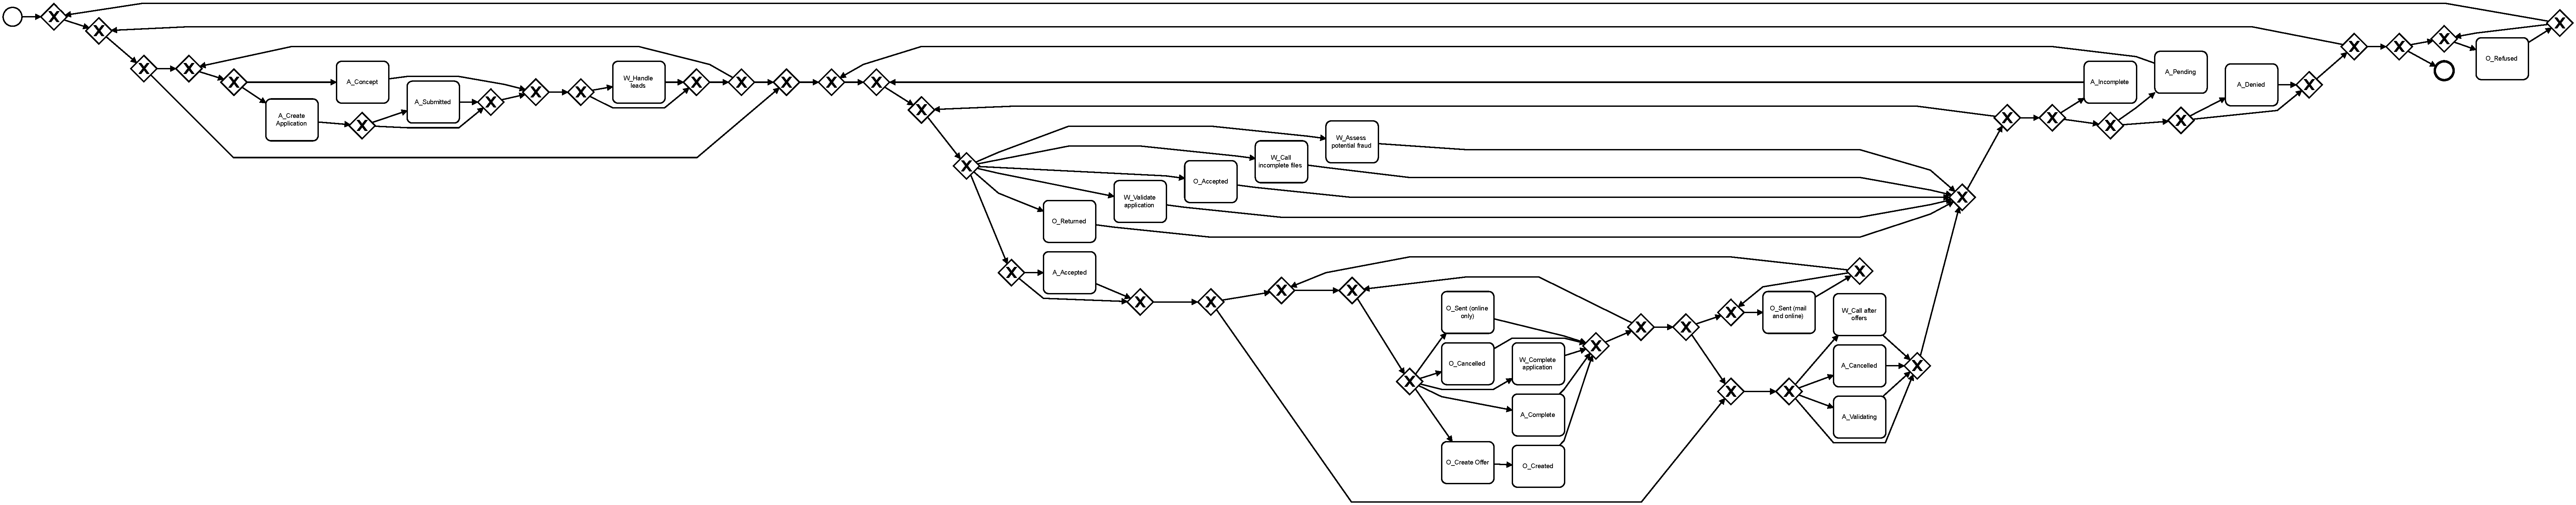
\includegraphics[width=\textwidth]{img/QUESTION_5b_BPMN_model.pdf}

% Second item
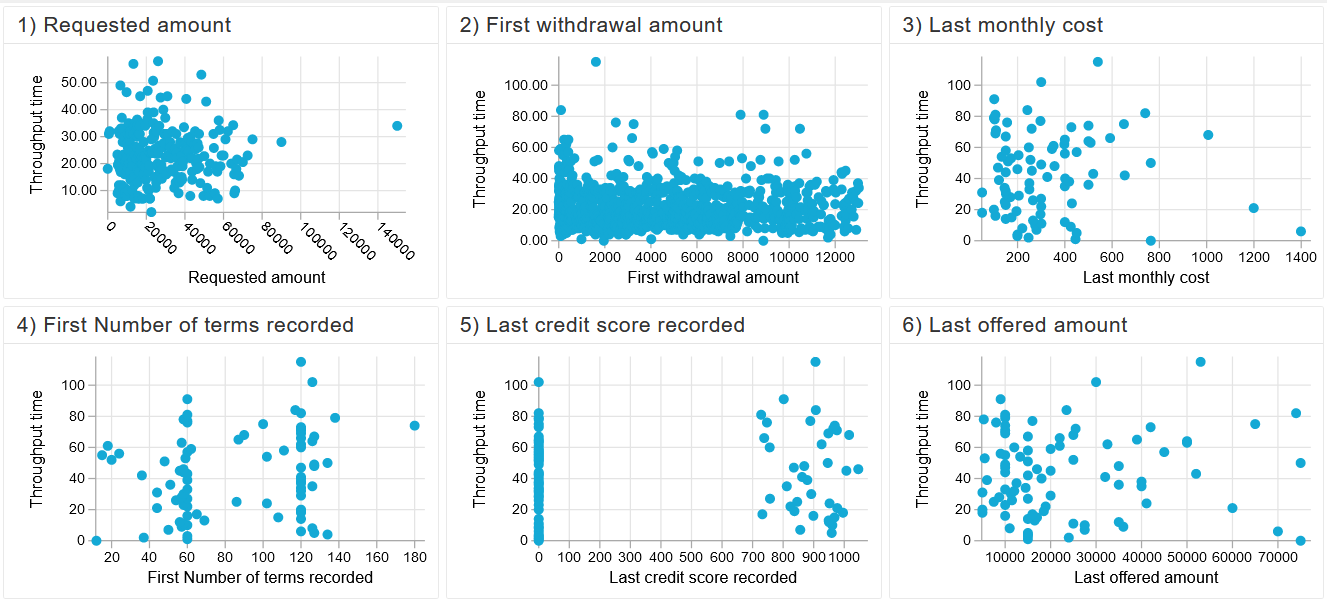
\includegraphics[width=\textwidth]{img/QUESTION_5b_scatter_plots.png}

% Third item
The DFG below was created by opening a new process explorer and only selecting the following activities to display: A$\_$Create $\_$Application, O$\_$Created, W$\_$Complete$\_$Application, O$\_$Accepted, O$\_$Refused, O$\_$Cancelled and A$\_$Cancelled. 100\% of activities and connections are being displayed. To see which edges are especially long-lasting we selected throughput time as our edge label.\\
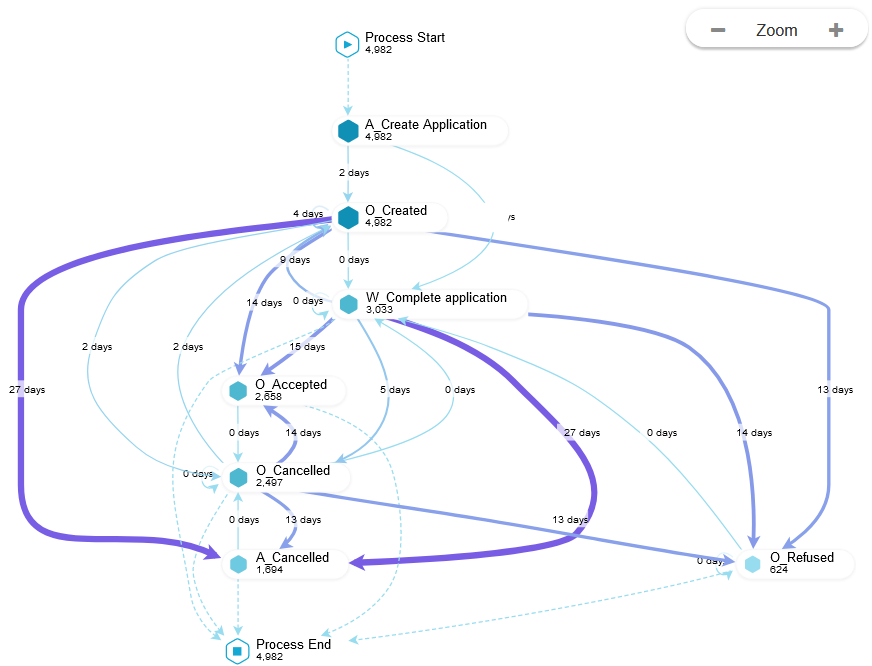
\includegraphics[width=\textwidth]{img/QUESTION_5b_DFG.png}
This way we can see that there are two very long-lasting edges (\texttt{O$\_$Created$\rightarrow$A$\_$Cancelled} and \texttt{W$\_$Complete$\_$application$\rightarrow$A$\_$Cancelled}) with a throughput time of 27 days. There is also a number of medium long-lasting edges with throughput times of 13-15 days

% Fourth item
The DFG below was created by opening a new process explorer and only selecting the following activities to display: A$\_$Create $\_$Application, O$\_$Created, W$\_$Complete$\_$Application, O$\_$Accepted, O$\_$Refused, O$\_$Cancelled and A$\_$Cancelled. 100\% of activities and connections are being displayed. We also filtered the dataset to only select cases with a throughput over 29 days.
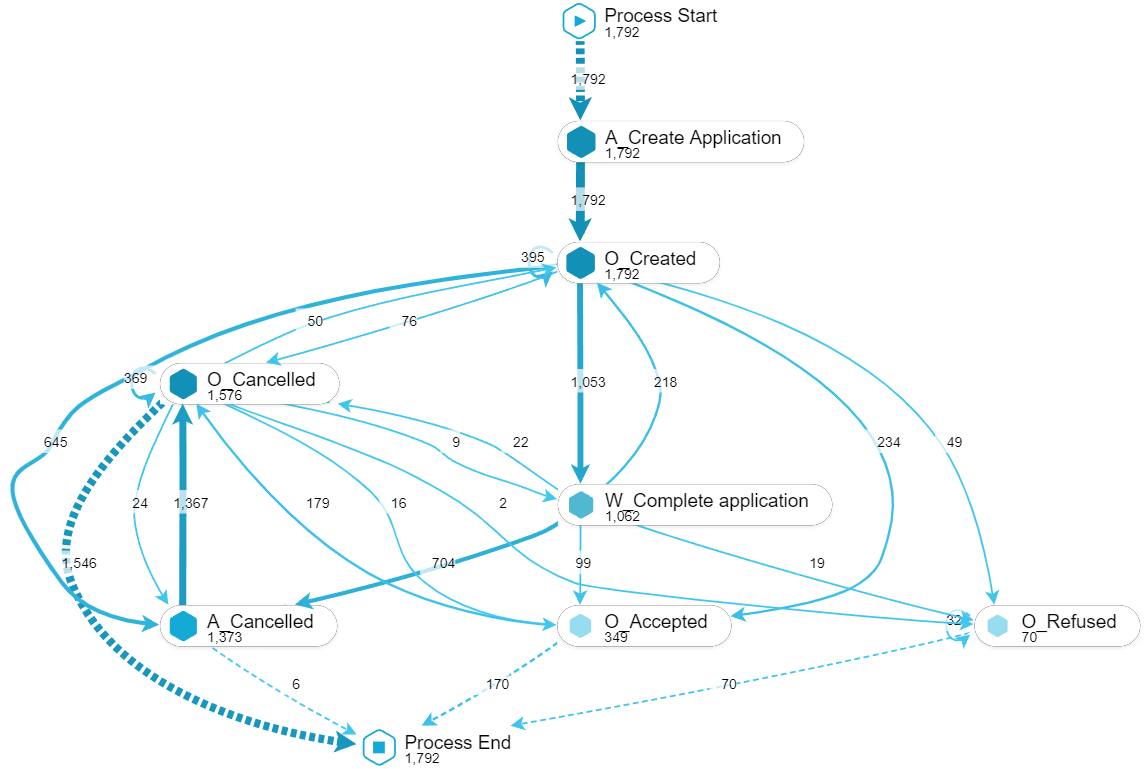
\includegraphics[width=\textwidth]{img/QUESTION_5b_over30.png}
Here we can see, that most cases with a throughput time over 29 days were cancelled. Additionally, most were passed through A$\_$Cancelled first, before passing through O$\_$Cancelled to the Process End.

\subsection*{(c)}
We open a new Process Overview for our Process in Celonis just like we did in a). To exclude all cancelled applications we add a new selection of type \textit{Attribute selection}. Since per definition cancelled applications are those that contain the activity \textit{A$\_$cancelled} we exclude all the applications containing it by selecting \texttt{Activity$\_$table$\_$csv > ACTIVITY > A$\_$Cancelled} and click \textit{Invert selection}. We also create a new throughput time selection for applications with a throughput time between 30 and infinity to only see long-running cases. The resulting Process Overview can be seen below.\\
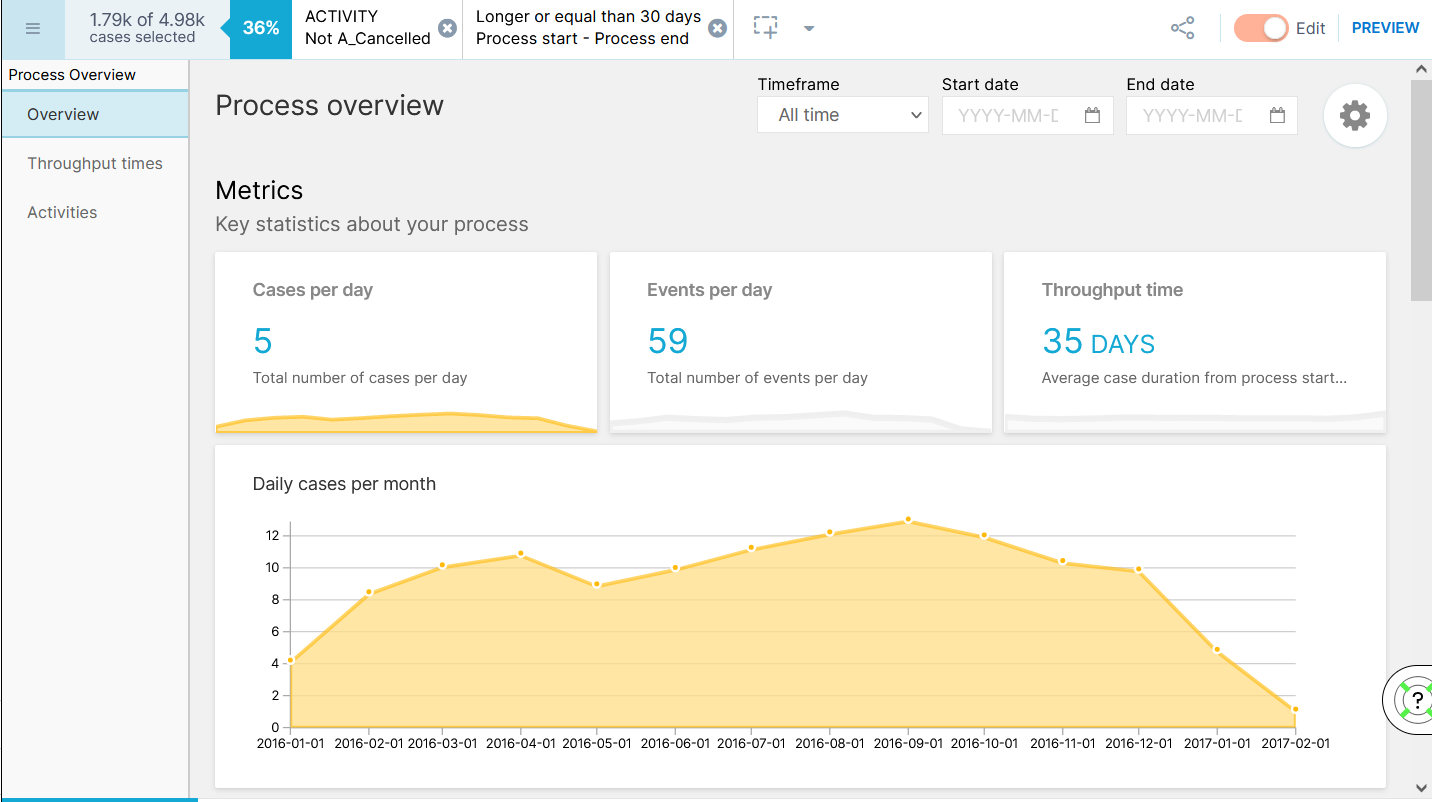
\includegraphics[width=\textwidth]{img/QUESTION_5c_process_overview.png}
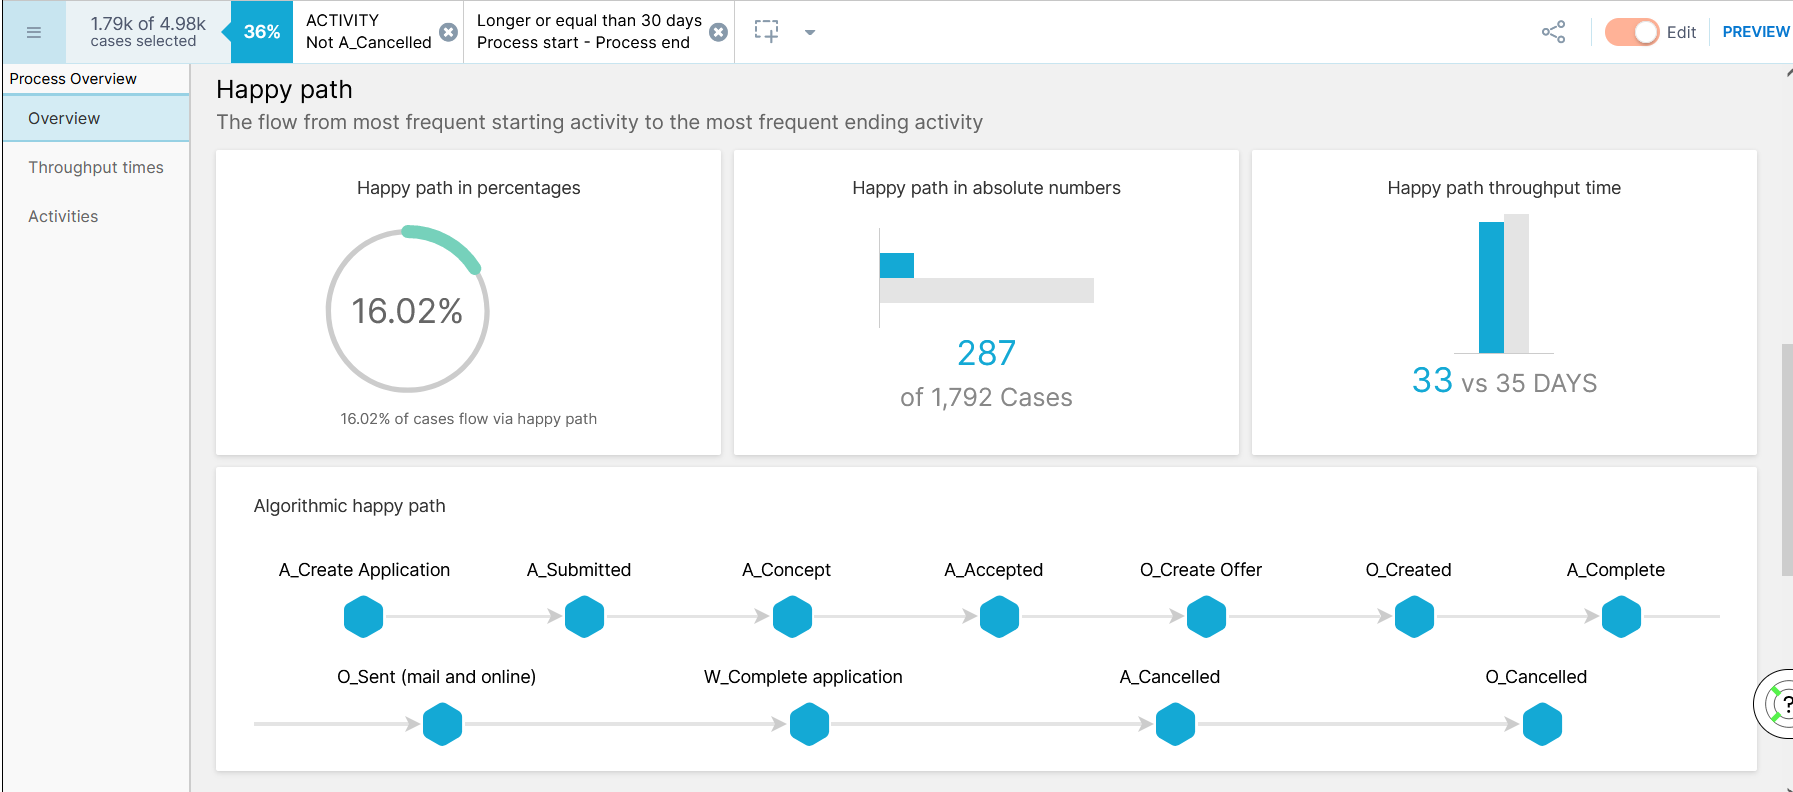
\includegraphics[width=\textwidth]{img/QUESTION_5c_process_overview_happy_path.png}
From it, we learn that there are 1792 long-running applications that weren't cancelled.


\subsection*{(d)}



\end{document}